
\documentclass[conference,letterpaper]{IEEEtran}
\usepackage[T1]{fontenc}
\usepackage[utf8]{inputenc}
\usepackage{times}
\usepackage{graphicx}
\usepackage{booktabs}
\usepackage[hidelinks,breaklinks]{hyperref}
\hypersetup{pdftitle={RESOLVE: Auditing Model Sensitivity in Lunar South-Polar Visibility Predictions},pdfauthor={RESOLVE project},pdfsubject={Technical Research Note}}
\pagestyle{plain}
\setlength{\emergencystretch}{1em}
\begin{document}
\title{RESOLVE: Auditing Model Sensitivity in Lunar South-Polar Visibility Predictions}
\author{\IEEEauthorblockN{RESOLVE project}\IEEEauthorblockA{Technical Research Note --- NASA Space Apps Challenge 2026\\Version 1.2 \enspace | \enspace 15 November 2026}}
\maketitle

\begin{abstract}

Lunar south-polar Sun/Earth visibility depends on terrain horizons, while a precise modeled duration can depend materially on terrain representation and other assumptions. RESOLVE audits whether a modeled landing-window result remains stable across defensible modeling choices. At dGR101, NASA Product 78 SL2 5 m gives 7.397830 days of complete simultaneous geometric Sun/Earth-center visibility; NASA Product 90 native 80 m gives 12.923283 days under the same fixed absolute observer convention, a difference of approximately +5.53 days. Frozen horizon and aligned terrain profiles identify a near-field representation mechanism. A limited negative result at dGR203 preceded this finding and redirected the investigation. These results establish a reproducible representation response, not an accuracy ranking. No terrain representation is validated as physical truth, and no fine-grid convergence plateau has been demonstrated. This note summarizes retained R-01A/B/C evidence; it introduces no new scientific calculation.

\end{abstract}

\begin{IEEEkeywords}Lunar terrain, geometric visibility, model sensitivity, decision auditing, scientific provenance.\end{IEEEkeywords}

\section{Introduction and research question}

RESOLVE was built for the NASA Space Apps Lunar Landing Site Navigator challenge. Near the lunar south pole, low solar elevations make local relief important to the terrain horizon. A precise visibility duration can therefore conceal sensitivity to terrain representation, observer position, event sampling or reporting scope. Candidate-site literature and its archive supplied comparison context and site coordinates [1].

The research question is: \textbf{Before a lunar landing-window prediction is relied upon, does the modeled answer remain stable under defensible changes in terrain representation and modeling assumptions?} Here, a ``window'' means a specified geometric-visibility interval, not an assessed landing opportunity with all mission constraints.

\section{Data and methods}

\subsection{Sources and geometry}
The retained experiments use NASA PGDA Product 78 local LOLA terrain and its official clones; Product 90 native 20/40/60/80/240 m terrain; and the separate Product 104 A304 image-enhanced Shape-from-Shading elevation model [2--6]. NASA/JPL NAIF SPICE supplies DE421 translation and the explicit MOON\_ME\_DE421 cartographic frame, with aberration convention NONE and a 1,737,400 m reference sphere [7]. The primary observable is simultaneous geometric visibility of the Sun and Earth centers above modeled terrain horizons. It does not calculate generated electrical power, a radio link budget, landing safety or mission certification.

\subsection{Matched observer and terrain}
At the archived dGR101 point\newline (latitude $-$88.5134116385092\textdegree{},\newline east longitude $-$68.01460926527753\textdegree{}), the primary observer is fixed at 1535.774658203 m above the reference sphere, defined by nominal P78 ground plus 2 m. Its height above each alternative represented surface therefore varies. A separate convention places the observer exactly 2 m above each surface and updates its absolute position consistently. Terrain replacement uses a common 20 $\times$ 20 km SL2 footprint; the existing native 80 m then 240 m exterior continuation remains fixed. Bilinear terrain interpolation and spherical curvature are retained; missing elevations are not replaced by zero [8].

\subsection{Intervals and refinement}
Registered-domain results use [6 November 2026 00:00, 28 November 2026 00:00 UTC). Complete results retain transition-bounded episodes intersecting that domain, with daily extension to discover actual boundaries. Frozen R-01C refinements halve angular/radial sampling and compare 150 s/75 s event discovery. Exact result rows, protocols, kernel/raster hashes and numerical audits remain accessible [8].

\begin{figure*}[!t]\centering
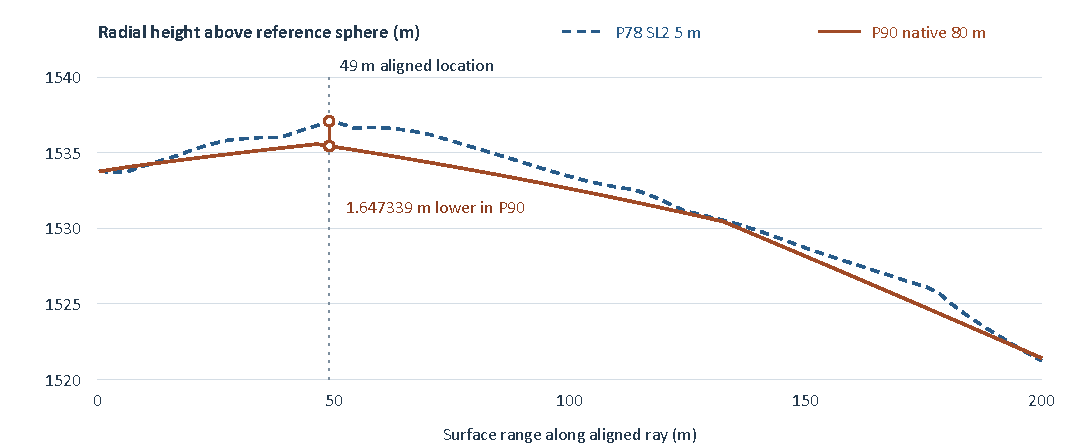
\includegraphics[width=0.95\textwidth]{RESOLVE_Technical_Research_Note_figure.pdf}
\caption{Aligned near-field profiles at the nominal P78 onset azimuth, 89.8356\textdegree{}. Vector redraw of the frozen P78/P90 section samples over their retained 0--200 m range; no terrain or visibility calculation was rerun. Heights are radial elevations above the 1,737,400 m reference sphere. Axes have different scales. The marked 49 m location differs from the 49.125 m own-event lower-bracketing witness below. Full original multi-product figures remain in the public evidence [8].}\label{fig:profile}\end{figure*}

\section{Research progression}

\textbf{R-01A: a hypothesis not supported.} The original hypothesis was that local stochastic terrain uncertainty could reverse the evaluated dGR203 6.5-day simultaneous-center classification. Nominal terrain and the first five official Product-78 clones retained the seasonal classification; the separate fixed-start grid also showed no terrain-driven classification reversal. This limited negative finding was retained, rather than treated as proof of zero terrain uncertainty [8].

\textbf{R-01B: a revised question.} A retained pre-outcome protocol specified a metadata-based multi-site screen after the dGR203 audit. That screen identified a large dGR101 response to a synthetic area-averaged 59.88 m local representation. A subsequent fixed-absolute-observer diagnostic was explicitly registered after detecting the contrast. The synthetic control is distinct from native NASA 60 m terrain. This sequence is falsification-driven research, not a result selected in advance [8].

\textbf{R-01C: native-product testing.} A further retained protocol tested the response using authoritative native Product-90 grids, a common absolute observer, complete intervals and numerical refinement. The several-day response persisted, showing that synthetic averaging alone did not account for the R-01B observation. Shared observations, geodetic ancestry and product processing preclude treating this as independent physical-truth validation [8].

\section{Results}

\begin{table}[!t]\centering
\caption{Longest complete simultaneous geometric Sun/Earth-center visibility episode intersecting the registered domain, at dGR101 under the primary fixed-absolute-observer convention. Values are reported to six decimal places from the frozen R-01C response table [8].}
\label{tab:result1}
\small\setlength{\tabcolsep}{6pt}\renewcommand{\arraystretch}{1.12}
\begin{tabular}{@{}lr@{}}\toprule
\textit{Terrain representation} & \textit{Complete window (d)}\\\midrule
P78 SL2 5 m & 7.397830\\
P90 native 20 m & 8.358389\\
P90 native 40 m & 9.676205\\
P90 native 60 m & 11.461184\\
P90 native 80 m & 12.923283\\
P90 native 240 m & 13.293702\\
P104 SDEM 5 m & 2.987840\\
\bottomrule\end{tabular}
\end{table}

The stored 80 m-minus-5 m contrast is 5.525453 days, approximately \textbf{+5.53 days}. The response is not a monotonic-convergence claim: native products differ in processing lineage and grid alignment as well as spacing. No fine-grid limiting window W* has been demonstrated; the retained 5 m-to-20 m complete-window difference is 0.960559 days. Product 104 is a separate product family, not another point on a single-resolution convergence sequence.

Observer and reporting definitions materially change interpretation. Product 104 gives 2.987840 days at the fixed absolute observer but 7.273578 days at 2 m above its own surface. Nominal P78 gives 5.379206 days when reporting-clipped, versus 7.397830 days for the complete episode. The clipped value cannot establish a physical failure of the 6.5-day benchmark.

\textbf{Numerical evidence.} The retained R-01C report records 29 software tests passing, a maximum accepted spatial transition/duration change of 327.157 s, and a maximum 150 s/75 s temporal change of 0.011926 s. Relevant event counts and scoped threshold states were stable. The preferred 60 s spatial target was not met in every check; the 600 s hard ceiling was met. These are deterministic consistency checks, not physical-accuracy bounds or confidence intervals [8].

\section{Physical mechanism}

At the nominal P78 solar-onset sector, the fixed-observer horizon is approximately \textbf{+1.537878\textdegree{}} in P78 and \textbf{$-$0.185233\textdegree{}} in native P90 80 m. Along the aligned ray at 49.000 m surface distance, P90 represents the terrain \textbf{1.647339 m lower} than P78. The retained near-field profiles therefore explain a lower represented skyline in this sector; they do not show that a physical lunar ridge disappears [8].

\begin{table*}[!t]\centering
\caption{Frozen own-event lower-bracketing witnesses, with a common absolute observer [8].}
\label{tab:result2}
\small\setlength{\tabcolsep}{6pt}\renewcommand{\arraystretch}{1.12}
\begin{tabular}{@{}lrrl@{}}\toprule
\textit{Representation} & \textit{Range} & \textit{Azimuth} & \textit{Own event (UTC, 2026)}\\\midrule
P78 SL2 5 m & 49.125 m & 89.8356\textdegree{} & 22 Nov 14:53:56.611\\
P90 native 80 m & 2.017 km & 151.0098\textdegree{} & 17 Nov 14:00:06.219\\
\bottomrule\end{tabular}
\end{table*}

\textbf{These own-event witnesses occur at different event times and azimuths. They are not two points on the same ray.} A horizon interpolates bracketing rays, and a witness is a sampled/interpolated terrain point rather than an independent laser return. The shared-azimuth profile and separate own-event witnesses are complementary diagnostics.

The duration contrast also includes a changed end boundary. For the late simultaneous episode, the frozen 80 m-minus-5 m onset shift is $-$5.037389 days and the end shift is +0.488064 days. The entire complete-window difference must not be assigned to one solar-onset ridge. All mechanism statements remain conditional on the matched geometry and represented terrain [8].

\section{Limitations}

No evaluated terrain representation is validated as physical truth, and no fine-grid convergence plateau is established. Product lineages differ in more than pixel spacing; pixel spacing is not effective independent terrain knowledge. The local high-resolution replacement retains a fixed coarser far-field continuation, so this is not a uniform-resolution lunar south-pole analysis. Numerical convergence tests address model consistency, not physical accuracy.

The exact DE441 effect remains unknown: a matched DE441 orientation/cartographic chain was not validated. The separate historical dGR203 approximately-seven-day literature discrepancy remains unresolved; unknown historical settings and an archived Sun-only/combined-product inconsistency prevent unique attribution. Product 104 shows strong observer-convention sensitivity. The dGR203 clone pilot contains only five local clones and is not a calibrated probability distribution. Limited sites and configurations do not support universal south-polar claims. No mission safety, certification, success probability or NASA endorsement is claimed [8].

\section{Implications}

A precise lunar visibility duration can remain model-sensitive across defensible terrain representations. Planning interfaces can benefit from exposing the stability of a result together with its assumptions, rather than presenting a duration alone. RESOLVE provides that audit for its evaluated cases, connects result changes to terrain-horizon evidence, and retains negative findings and unresolved limits. Broader applicability requires separately specified evidence.

\newpage

\section{Reproducibility and data availability}

Live interface: \href{https://resolve-lunar-audit.vercel.app/}{resolve-lunar-audit.vercel.app}. Source and released product records: \href{https://github.com/MangoMuffinLover/resolve-lunar-audit}{GitHub repository}. Protocols, findings, numerical audits, exact CSVs, source hashes and reproduction instructions: \href{https://resolve-lunar-audit.vercel.app/science/}{Science \& Evidence}. This note summarizes the frozen evidence retained in release 324d5b6a8d8b6cdd99a3d5ed314e5874268cb4de; it adds no new research run.

The public repository reproduces the interface from included frozen product records; it does not contain the full raw DEM/SPICE research environment. Full scientific reproduction needs the specified retained raw inputs, kernels and research code. Acquired native-window and byte-range checksums are scoped to those bytes, not unknown whole-remote-raster digests. The note's editable source, builder and file hashes accompany the release. AI assisted drafting and software development; numerical claims here are attributed to retained computational evidence.

\begin{thebibliography}{8}
\bibitem{ref1} Wueller et al. (2026). Assessing Potential Landing Sites With Favorable Illumination and Accessible, Potentially Volatile-Rich Permanently Shadowed Regions Within Artemis Candidate Landing Regions. \href{https://doi.org/10.1029/2025JE009434}{10.1029/2025JE009434}. Candidate archive: \href{https://doi.org/10.5281/zenodo.17084058}{10.5281/zenodo.17084058}.
\bibitem{ref2} NASA GSFC PGDA. \href{https://pgda.gsfc.nasa.gov/products/78}{Product 78: High-Resolution LOLA Topography for Lunar South Pole Sites}.
\bibitem{ref3} NASA GSFC PGDA. \href{https://pgda.gsfc.nasa.gov/products/90}{Product 90: A New View of the Lunar South Pole from LOLA}.
\bibitem{ref4} Barker et al. (2023). A New View of the Lunar South Pole from LOLA. \href{https://doi.org/10.3847/PSJ/acf3e1}{10.3847/PSJ/acf3e1}.
\bibitem{ref5} NASA GSFC PGDA. \href{https://pgda.gsfc.nasa.gov/products/104}{Product 104: Enhanced Topography Models for Selected Lunar South Pole Regions with Shape-from-Shading}.
\bibitem{ref6} Bertone et al. (2026). Enhanced Topography Models for Selected Lunar South Pole Regions with Shape-from-Shading. The Planetary Science Journal. \href{https://doi.org/10.3847/PSJ/ae5b70}{10.3847/PSJ/ae5b70}. \href{https://ntrs.nasa.gov/citations/20260004665}{NASA NTRS record 20260004665}.
\bibitem{ref7} NASA/JPL NAIF. \href{https://naif.jpl.nasa.gov/pub/naif/generic_kernels/fk/satellites/moon_080317.tf}{Lunar frame definitions}; \href{https://naif.jpl.nasa.gov/pub/naif/generic_kernels/spk/planets/a_old_versions/}{archived planetary ephemerides including DE421}.
\bibitem{ref8} RESOLVE frozen R-01A/B/C evidence: findings, protocols, R-01C response/witness tables, numerical audit, source/frame/literature audits and reproduction instructions. \href{https://resolve-lunar-audit.vercel.app/science/}{Public evidence index}. Specific input paths and SHA-256 values are listed in the accompanying note provenance record.
\end{thebibliography}\end{document}
